\documentclass[10pt, a4paper]{beamer}

\usetheme{Berkeley}
\usecolortheme{sidebartab}
\usepackage{graphicx}
\graphicspath{{images/}}

\begin{document}
	\setbeamertemplate{sidebar left}{}
	\title{Progress Presentation-I}
	\subtitle{e-Yantra Summer Internship 2017 \\ \bfseries Control and Algorithms Development for Quadcopters}
	\author{Heethesh Vhavle\\
	Mentors: Sanam Shakya $|$ Pushkar Raj}
	\institute{IIT Bombay}
	\date{\today}
	%\addtobeamertemplate{sidebar left}{}{\includegraphics[scale = 0.3]{logowithtext.png}}
	\frame{\titlepage}

\setbeamertemplate{sidebar left}[sidebar theme]
\section{Overview of Project}
\begin{frame}{Overview of Project}
\bfseries Control and Algorithms Development for Quadcopters \\
\hfill \break
\mdseries 
\begin{itemize}
\item To develop custom firmware for quadcopter for 32-bit microcontrollers on STM32F1xx (ARM Cortex-M3 core).\\
\item Control parameters such as the throttle, yaw, pitch and roll and to develop algorithms considering various motion and dynamics.\\
\item To analyse the control algorithm to identify effects of various parameters and to optimize it for stable motion.\\
\item Develop a wireless joystick controller for maneuvering of the quadcopter. 
\end{itemize}
\end{frame}

\section{Overview of Task}
\begin{frame}{Overview of Task}
\begin{tabular}{|l|p{0.6\linewidth}|p{0.15\linewidth}|} 
\hline
Task No. & Task & Deadline\\ \hline
1 & Study of datasheet and user guide of Pluto Drone. & 2 days\\ \hline
2 & Installation and Setup of IDE and tools. & 1 day\\ \hline
3 & Libraries development for GPIO, Timers, PWM, UART, I2C interface. Interfacing IMU to obtain filtered pitch, roll and yaw angles. & 3+4 days\\ \hline
4 & Code development for control of quadcopter for stable flight. & 12 days\\ \hline
5 & Wireless joystick control (using Node MCU). & 6 days\\ \hline
6 & Documentation for testing and debugging the drone. & 6 days\\ \hline
\end{tabular}
\end{frame}

\section{Task Accomplished}
\begin{frame}{Task Accomplished}
\bfseries Task 1\\ Study of datasheet and user guide of Pluto Drone\\ \hfill \break
\mdseries 
\begin{itemize}
\item Brief study on the ARM Cortex-M3 architecture to understand how the various peripherals (such as the timers, GPIO ports, I2C ports) have been interfaced the APB.\\ 
\item Study of the clock distribution (RCC) and configuration of various clock sources.\\
\item Brief study of existing flight controllers such as CleanFlight  and Naze32 for 32-bit micro-controllers.
\end{itemize}	
\end{frame}

\begin{frame}{Task Accomplished}
\bfseries Task 2\\ Installation and Setup of IDE and tools\\ \hfill \break
\mdseries 
\begin{itemize}
\item Successfully installed TrueSTUDIO IDE, GNU ARM Tool-chain, Windows Build Tools, OpenOCD, Device Packs and Drivers for STM32F10xx.\\
\item Hardware debugging was successfully completed.
\end{itemize}	
\end{frame}

\begin{frame}{Task Accomplished}
\bfseries Task 3\\ Libraries development for GPIO, Timers, PWM, UART, I2C interface\\
\mdseries 
\begin{itemize} 
\item Developed libraries for GPIO pin control.\\
\item Configured timers for PWM control of motors.\\
\item Serial communication over UART for various data types.\\
\item I2C port was configured for sensor interfacing.\\
\item MPU9250 Accelerometer and Gyroscope was interfaced.\\ 
\item AK8963 Magnetometer was also interfaced.\\ 
\item Finding the yaw angle required a more complex algorithm and this was achieved using Madgwick's AHRS filter. 
\item However, the angles obtained are not yet accurate due to certain problems with Accelerometer interfacing.
\end{itemize}
\end{frame}

\begin{frame}{Task Accomplished}
\bfseries Sensor Calibration and Data Visualization\\ \hfill \break
\mdseries 
\begin{itemize} 
\item The MPU9250 and AK8963 sensors were calibrated for offsets. 
\item The calibrated data was visualized using Python. 
\item Currently working on real time data visualization using Python. Successfully implemented data frame transmission with checksum. 
\item Process of plotting the real time data and development of a GUI is ongoing.
\end{itemize}
\end{frame}

\begin{frame}{Task Accomplished}
\bfseries Calibration Process\\ \hfill \break
\mdseries 
\begin{itemize} 
\item Around 6,000 raw data samples were recorded.
\item Average offset value was calculated as (MAX + MIN)/2 for all axes.
\item Scaling factor was calculated as (MAX - MIN)/2 and then normalized.
\item 3D scatter plots for all axes were visualized in Python.
\end{itemize}
\end{frame}

\begin{frame}{Task Accomplished}
\begin{center}
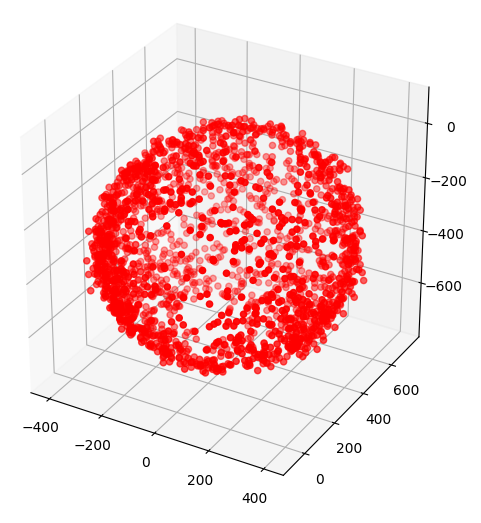
\includegraphics[scale=0.45]{raw}\\
Raw Data from AK8963 Magnetometer
\end{center}
\end{frame}

\begin{frame}{Task Accomplished}
\begin{center}
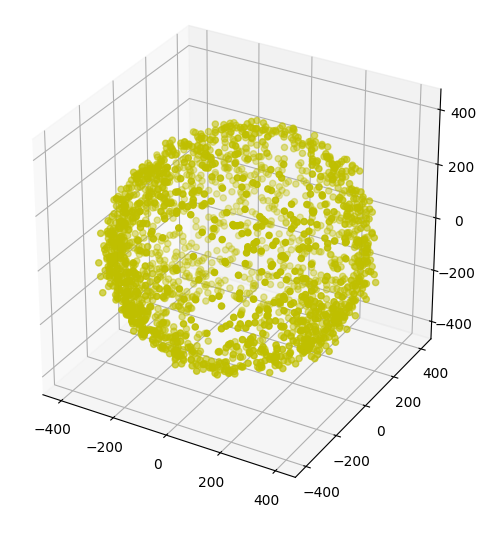
\includegraphics[scale=0.45]{offset}\\
Offset Corrected Data
\end{center}
\end{frame}

\begin{frame}{Task Accomplished}
\begin{center}
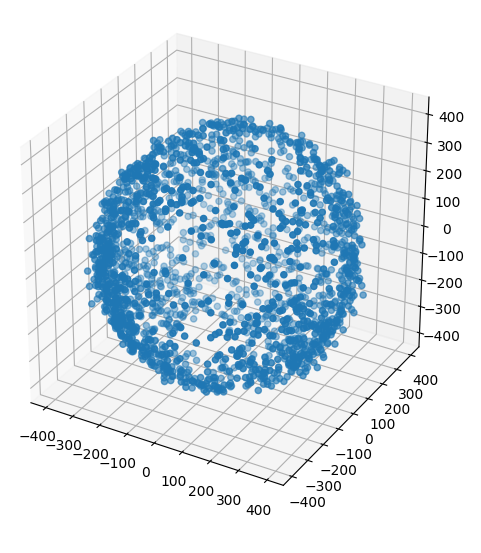
\includegraphics[scale=0.45]{scaled}\\
Scaled and Offset Corrected Data
\end{center}
\end{frame}

\section{Challenges Faced}
\begin{frame}{Challenges Faced}
\begin{itemize}
\item One of the main challenges was developing libraries for peripheral interfaces because of the vast array of documentation and software libraries to wade through [Solved].\\
\item Sensor calibration to obtain accurate data which is required for sensor fusion [Solved].\\
\item Interfacing the AK8963 magnetometer on the same I2C bus as that of the MPU9250 [Solved].\\
\item Abrupt changes in the accelerometer data due to which angles computed are not stable [Debugging].
\end{itemize}
\end{frame}

\section{Future Plans}
\begin{frame}{Future Plans}
\begin{itemize}
\item Perfectly calibrated pitch, roll and yaw with real-time data visualization (with GUI).\\
\item Initial control algorithms for pitch, roll, yaw and throttle control will be developed.\\
\item Barometer and VL53L0X ranging sensor interface for stable altitude control.
\end{itemize}
\end{frame}


\section{Thank You}
\begin{frame}{Thank You}
	\centering THANK YOU !!!
\end{frame}
\end{document}
